\subsection{Dark Matter}
The effects of dark matter are apparent through a few observations.
The most notable come from observed galaxy formation, gravitational lensing, and the missing power seen in the cosmic microwave background power spectrum \cite{DM_Hist}.
Aside from these large scale observations, dark matter is extremely difficult to detect experimentally with no known exact form.
Current theory introduced two popular candidates: axions and weakly interacting massive particles (WIMPs) \cite{DM_Hist}.
The XENON Collaboration aimed to directly detect WIMPs using the XENON1T experiment.
The collaboration has moved on to the successor XENONnT, but the topics discussed here will with regard to XENON1T.

\subsection{XENON1T Detector}
The XENON1T detector is a dual phase xenon time projection chamber (TPC) located in the \textit{Laboratori Nazionali del Gran Sasso} (LNGS) in central Italy.
It was a requirement for the detector to be sensitive to keV energy levels in order to detect WIMPs, so the detector's placement in LNGS, use of xenon, and water shielding were all necessary components to the experiment \cite{Xenon1t}.
It contains a fiducial mass of $\sim$1.3 tons of liquid xenon and a fiducial volume with a maximum radius of 42.84 cm \cite{1TDM_DataAnalysis}.
The detector features 258 photomultiplier tubes (PMTs): 127 on the top array and 121 on the bottom array.
\begin{wrapfigure}{r}{0.5\textwidth}
	\centering
	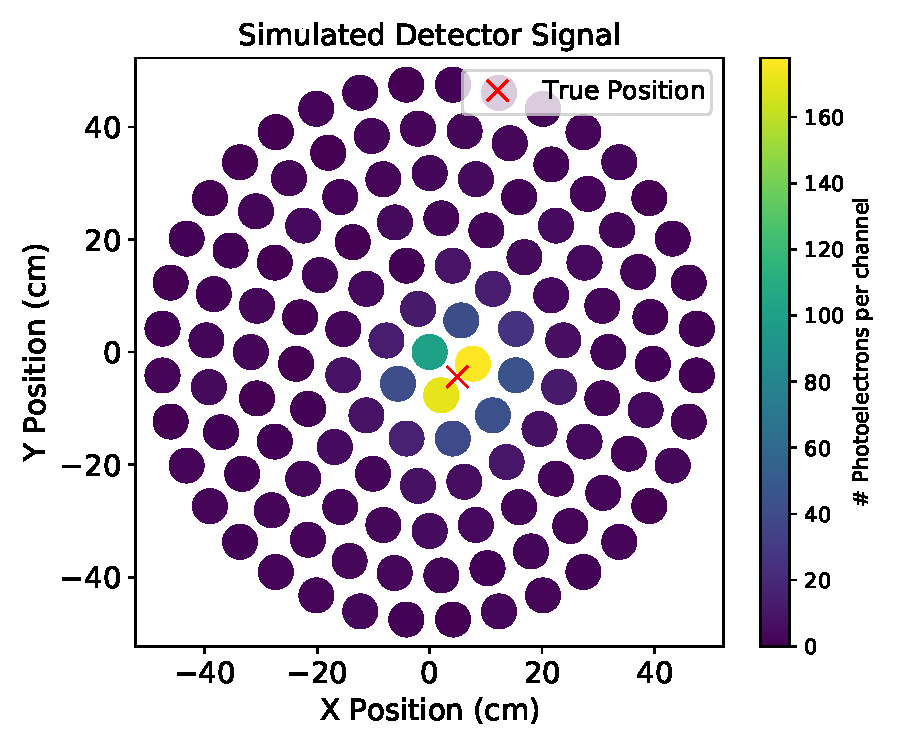
\includegraphics[width=\linewidth]{figures/opt_sim_hit_989.pdf}
	\caption{Example simulated hit pattern.
	Each circle represents a PMT in the top array of the detector.
	The position of each circle is the real position of the PMT in the detector.
	The simulation has a true position marked by the red x and created the shown hit pattern.}
	\label{fig:example_hit}
\end{wrapfigure}
\pdfmarkupcomment[markup=Highlight, color=yellow]{There is a constant electric field of 116.7 V/cm that causes electrons to drift towards the liquid-gas interface at the top of the detector, where they are extracted by a stronger electric field and produces a proportional scintillation signal}{Feels very awkward. Also seems close to the introduction of the citation.} \cite{Xenon1t}.

\par An event in the detector occurs when a particle scatters off xenon atoms.
The recoil energy results in a scintillation and ionization from these xenon atoms.
The scintillation is observed by the PMTs and regarded as the S1 signal.
The signal produced by the ionization at the liquid-gas interface is regarded as the S2 signal.
An example of this signal is shown in Figure \ref{fig:example_hit}.
Using the light pattern of the S2 signal from the top array of PMTs, we are able to reconstruct the $(x, y)$ position of the event in reference to the plane of the PMTs.
This process is referred to as \textit{position reconstruction}.

\par Using the reconstructed positions, we're able to filter out terabytes of data by excluding events that are outside the fiducial volume.
However, implementations of position reconstruction, such as maximum PMT, weighted sum position, multilayer perceptron, have pitfalls of reconstructing outside the detector, being inaccurate, or both \cite{Bart}.
For us to get accurate results, we want an algorithm to have a standard deviation for the Euclidean distance between reconstructed position and true position to be less than the space between PMTs (0.35 cm).
\subsection{Machine Learning}
The maximum PMT and weighted sum position algorithms were two cases that did well to keep reconstructions within the detector walls.
However, these algorithms did not do well for their overall accuracy.
One of the initial machine learning algorithms that was applied a neural network.
Recently, this neural network takes the form of a multilayer perceptron.
These neural networks have performed significantly better in terms of their overall accuracy, but have difficulty keeping the reconstructions within the bounds of the detector.
It is difficult to encode the detector walls into the neural network while also maintaining their good accuracy.
This difficulty at the walls is due to the hard cut off of information.
There are no more PMTs and thus there is no information present to inform the network that nothing is occurring outside the detector.
At the same time, experimental data will hold many problems.
The observed S2 signal is not clean, as in background events are present within the S2 signal.
Over the course of the experiment, PMTs will break and the signal they would see can no longer be used.
